% !TeX program = latexmk
\documentclass[11pt,a4paper]{article}
\usepackage[utf8]{inputenc}
\usepackage[T1]{fontenc}
\usepackage{lmodern}
\usepackage{geometry}
\geometry{margin=1in}
\usepackage{xcolor}
\usepackage{hyperref}
\hypersetup{
  colorlinks=true,
  linkcolor=blue,
  citecolor=teal,
  urlcolor=magenta,
  pdftitle={MCP Security},
  pdfauthor={Yusuf Arabci et al.}
}
\usepackage{graphicx}
\usepackage{tikz}
\usetikzlibrary{arrows.meta,positioning,fit}
\usepackage{csquotes}
\usepackage{booktabs}
\usepackage{enumitem}
\usepackage{microtype}
\usepackage[backend=biber,style=numeric,sorting=none]{biblatex}
\addbibresource{bibliography/references.bib}

\title{Model Context Protocol (MCP) Security:\\ Threats, Defenses, and Deployment Guidance}
\author{Yusuf Ar\"{a}b\c{c}\i{} et al.}
\date{\\Draft: \today}

\begin{document}
\maketitle
\begin{abstract}
We study the security landscape of the Model Context Protocol (MCP), outlining threat models, attack classes, and practical defenses for safe deployments.\\
This is a working draft prepared with \LaTeX{} and VS Code.
\end{abstract}

\section{Introduction}
% Intro\nThis paper investigates MCP security, contributions: (i) structured threat model, (ii) taxonomy of attacks, (iii) actionable defenses and deployment guidance.

\section{Background}
MCP, LLM tabanlı uygulamalar için araç ve veri erişimini ortak bir protokole soyutlayarak; MCP istemcisi (LLM uygulaması), bir veya daha fazla MCP sunucusu (araç/ kaynak vekili) ve harici araç/hizmet rollerini tanımlar. Taşıma çoğunlukla JSON-RPC benzeri kanallar üzerinden gerçekleşir.

Temel Bileşenler
- İstemci: İstek üretir, oturum bağlamını yönetir, UI/UX ilkelerini uygular.
- Sunucu: Araç ve veri kaynaklarını tekdüze bir arabirim üzerinden sunar, yürütmeyi aracılar.
- Araç/Hizmet: Dosya sistemi, HTTP API, veritabanı gibi farklı risk profillerine sahip eylemler.

Güven sınırları: İstemciler sunucu/araçları varsayılan olarak güvenilir saymamalı; sunucu araçları politikalarla kısıtlamalı; araçlar mümkün olduğunca yalıtılmalıdır.

\begin{figure}[h]
\centering
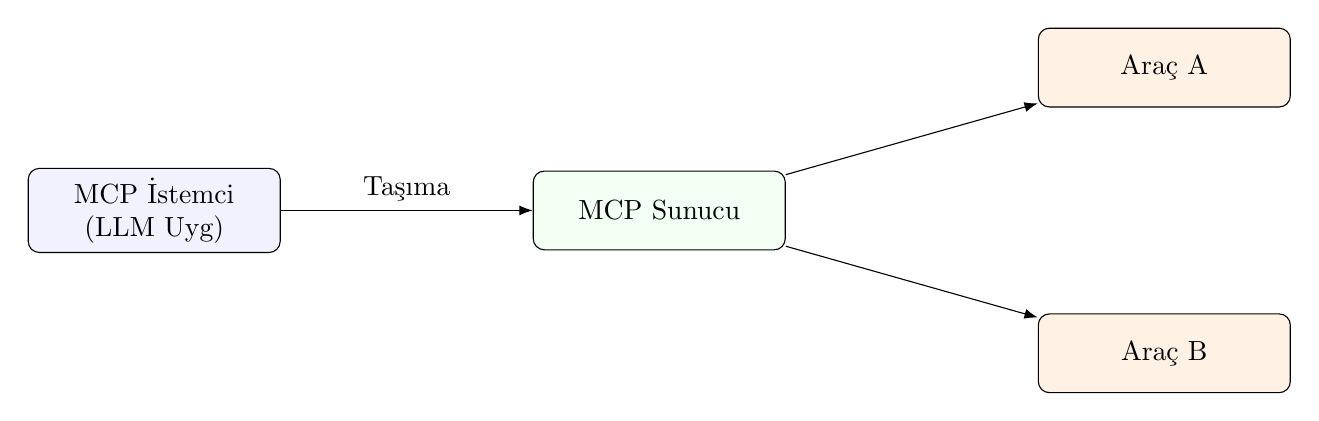
\begin{tikzpicture}[
  comp/.style={rectangle,draw,rounded corners,align=center,minimum width=3.2cm,minimum height=1cm},
  arr/.style={-Latex}
]
\node[comp, fill=blue!5] (client) {MCP İstemci\\(LLM Uyg)};
\node[comp, fill=green!5, right=3.2cm of client] (server) {MCP Sunucu};
\node[comp, fill=orange!10, above right=0.8cm and 3.2cm of server] (tool1) {Araç A};
\node[comp, fill=orange!10, below right=0.8cm and 3.2cm of server] (tool2) {Araç B};
\draw[arr] (client) -- node[above]{Taşıma} (server);
\draw[arr] (server) -- (tool1);
\draw[arr] (server) -- (tool2);
\end{tikzpicture}
\caption{Basitleştirilmiş MCP topolojisi ve güven sınırları.}
\label{fig:mcp-arch}
\end{figure}

Operasyonel Bağlam
- Kurulumlar yerel geliştirici ortamlarından (yüksek ayrıcalık, düşük yalıtım) çok kiracılı bulut dağıtımlarına (sıkı yalıtım ve denetleme) kadar çeşitlenir.
- Açık sunucu ve zayıf kimlik doğrulama/yetkilendirme gibi yanlış yapılandırmalar maruziyeti ciddi biçimde artırır \cite{MDPIElectronics3267}.


\section{Threat Model}
Varlıklar
- Gizli veriler: API anahtarları, kimlik bilgileri, müşteri/kurumsal veriler.
- Eylem bütünlüğü: araç çağrıları, dosya değişiklikleri, yürütme çıktıları.
- Kullanılabilirlik: istemci/sunucu çalışma süresi, oran ve bütçe sınırları.

Saldırganlar
- Ağ üzerinden dış aktör.
- Kötü niyetli/ele geçirilmiş araç veya sunucu sağlayıcı (tedarik zinciri).
- İç tehdit veya ele geçirilmiş işletim/uç nokta.

Varsayımlar
- Taşıma katmanı gizlilik/bütünlük sağlar (TLS), ancak uçlar güvenilir olmayabilir.
- Modeller halüsinasyon üretebilir; içerik veya araç meta verisi yoluyla prompt enjeksiyonu mümkündür.
- Araçların etki alanı farklıdır (dosya sistemi > salt-okunur HTTP gibi).

Güvenlik hedefleri
- Gizlilik: sırların araç yanıtları ve günlükler ile sızmaması.
- Bütünlük: yetkisiz/istenmeyen yan etkilerin önlenmesi.
- Kullanılabilirlik: kaynak kullanımını sınırla; saldırı altında güvenli bozulma.

Güven Sınırları
- İstemci $\leftrightarrow$ Sunucu: kimlik doğrulama, yetkilendirme, yetenek/kapasite mutabakatı.
- Sunucu $\leftrightarrow$ Araçlar: yalıtım ve politika uygulama.
- Kullanıcı $\leftrightarrow$ Model: prompt hijyeni, içerik filtreleme, kullanıcı onayı.


\section{Vulnerabilities and Attacks}
Saldırı sınıflarını ana vektör ve etkilerine göre grupluyor, güncel vakalarla örneklendiriyoruz.

Prompt/Tool Poisoning
- Araç tanımlarına veya yanıtlarına gömülü kötü talimatlar, modeli veri sızıntısı veya riskli eylemlere yöneltebilir. Etkiler: kimlik bilgisi sızdırma, politika atlatma \cite{arXiv250323278,arXiv250812566}.

Plan Enjeksiyonu
- ReAct, Tree-of-Thoughts gibi çok adımlı akıl yürütme yöntemleri; ara içeriklerle sonraki adımların saptırılması ve kademeli ayrıcalık artışı için hedef alınabilir \cite{arXiv250907595}.

Uzaktan Kod Çalıştırma (RCE)
- Güvensiz komut inşası, serileştirme veya aşırı ayrıcalıklı araçlar, sunucu/host üzerinde keyfi kod çalıştırmaya yol açar.

Ağ Pivotu (SSRF/DNS Rebinding)
- Ağ I/O yapan araçlar, iç servisler veya metadata uç noktalarına erişim için kötüye kullanılabilir; DNS rebinding köken varsayımlarını bozar.

Kimlik Doğrulama/Yetkilendirme Açıkları ve Açık Sunucular
- Kimlik doğrulaması veya yetenek kapsamı olmadan erişime açılan MCP sunucuları ile sınırsız sorgu ve veri erişimi mümkün olur \cite{MDPIElectronics3267}.

Tedarik Zinciri ve Typosquatting
- Kötü amaçlı paketler veya sunucu güncellemeleri arka kapı yerleştirebilir; aşağı akıştaki istemcileri etkiler.

\begin{table}[h]
\centering
\begin{tabular}{@{}lll@{}}
\toprule
Saldırı Sınıfı & Tipik Vektör & Birincil Etki \\
\midrule
Tool/Prompt Poisoning & Güvenilmeyen meta veri/içerik & Veri sızıntısı, politika atlatma \\
Plan Enjeksiyonu & Yinelemeli akıl yürütme çıktıları & Yetkisiz eylem, ayrıcalık artışı \\
RCE & Aşırı ayrıcalıklı araçlar, güvensiz exec & Host ele geçirilmesi \\
SSRF/DNS Rebinding & Ağ yetenekli araçlar & İç veri erişimi, pivot \\
AuthN/Z Açıkları & Açık/zayıf korumalı sunucular & Sınırsız sorgu \\
Tedarik Zinciri & Kötü paketler/güncellemeler & Yaygın kompromizasyon \\
\bottomrule
\end{tabular}
\caption{MCP saldırı sınıfları ve etkileri (tam değildir).}
\label{tab:attacks}
\end{table}


\section{Defenses and Best Practices}
Katmanlı Savunma
- Yalıtım ve Sandboxing: araçları OS seviyesinde izole edin (container, namespace); ayrıcalıkları düşürün; dosya sistemi ve ağ çıkışını varsayılan olarak kısıtlayın.
- En Az Ayrıcalık: açık ve dar yetenek setleri; varsayılan olarak reddet; oturum kapsamlı kimlik bilgiler.
- Doğrulama ve Kısıtlama: girdi/çıktı sanitizasyonu; komut/API beyaz listeleri; prompt/tool poisoning için içerik filtreleri.
- Gözlemlenebilirlik: yapılandırılmış loglar, izleme (örn. OpenTelemetry), anomali tespiti; sırları maskeleyin.
- Oran Sınırlama ve Bütçeler: oturum/kullanıcı başına istek, süre ve maliyeti sınırlandırın.

Protokol Düzeyi (Seçenekler)
- Yetenek Tanımlayıcıları: araç izinleri ve yan etkilerinin makinece okunur beyanları.
- İmzalama ve Doğrulama: imzalı araç manifestleri; istemciye sunucu kimlik doğrulaması.
- Oturum Kapsamı: kimlik bilgilerini ve depolamayı kullanıcı/oturum bazında sınırlandırın.

Operasyonel Rehber
- Maruz Yüzey: MCP sunucularını kimlik doğrulamasız yayımlamayın; ağ geçidi arkasında konumlandırın; sırları düzenli döndürün.
- Konfigürasyon Hijyeni: sürüm kontrollü ve gözden geçirilmiş konfigürasyon; açık beyaz listeler; güvenli varsayılanlar.
- Test: araçlar için güvenlik regresyon testleri; prompt ve girdi işleme için fuzzing.


\section{Related Work}
Ajan çatıları ve eklenti ekosistemlerinde belgelendirilen riskler MCP’ye de genellenir: prompt enjeksiyonu ve tool poisoning, yetersiz yalıtım ve tedarik zinciri maruziyeti \cite{arXiv250323278,arXiv250812566}. Operasyonel çalışmalar, açık servislerde yanlış yapılandırmaların yaygınlığını ve en az ayrıcalık ile izlemenin önemini vurgular \cite{MDPIElectronics3267}. Yakın tarihli araştırmalar, araç çağrıları için işlev‑olarak‑hizmet (FaaS) temelli dayanıklı iş akışlarının ayrıcalık alanını küçültebileceğini ve yalıtımı sadeleştirebileceğini göstermektedir \cite{arXiv250907595}. Alan‑özgü öneriler (örn. biyoinformatik) yetenek kapsamı ve denetimin güvenli entegrasyonu nasıl desteklediğini örneklemektedir \cite{arXiv250708055}.


\section{Conclusion}
% Conclusion and future work.


\printbibliography
\end{document}
